\documentclass[a4paper,12pt]{article}
% if you need additional LaTeX packages, add them here
\usepackage[]{geometry}
\usepackage{graphicx, wrapfig, enumitem}
\usepackage{subcaption}
\usepackage{xcolor}
\usepackage{listings, ulem}
\usepackage[most]{tcolorbox}
\usepackage{multirow, multicol, tabularx, booktabs}
\usepackage{fancyhdr}
\usepackage{tikz}
\usepackage{hyperref}
\usepackage[simplified]{pgf-umlcd}
\usepackage{subfiles}
\usepackage[linguistics]{forest}
\usepackage{caption}
\usepackage{circuitikz}
\usepackage{tcolorbox}

\graphicspath{{Resources/}}

\setlist{nolistsep}
\setlength{\parindent}{0in}


\usetikzlibrary{decorations.markings}
\usetikzlibrary{calc}
\tikzset{middlearrow/.style={
        decoration={markings,
            mark= at position 0.5 with {\arrow{#1}} ,
        },
        postaction={decorate}
    }
}
\def\centerarc[#1](#2)(#3:#4:#5)% Syntax: [draw options] (center) (initial angle:final angle:radius)
    { \draw[#1] ($(#2)+({#5*cos(#3)},{#5*sin(#3)})$) arc (#3:#4:#5); }



\hypersetup{colorlinks=true, linkcolor=blue!50!red, urlcolor=green!70!black}

% defining a warning box
\definecolor{orang}{RGB}{255,155,0}

\newtcolorbox[auto counter,number within=section]{warningbox}[1][]{
  enhanced jigsaw,colback=white,colframe=orang,coltitle=orang,
  fonttitle=\bfseries\sffamily,
  sharp corners,
  detach title,
  leftrule=22mm,
  % What you need %%%%%%%%%%%%
  underlay unbroken and first={\node[below,text=black,anchor=east]
  at ([xshift=-22.5pt]interior.base west) {\Huge  \textbf{!}};},
  %%%%%%%%%%%%%%%%%%%%%%%%
  breakable,pad at break=1mm,
  #1,
  code={\ifdefempty{\tcbtitletext}{}{\tcbset{before upper={\tcbtitle\par\medskip}}}},
}

\newenvironment{centerdiagram}[1][\topsep]
  {\setlength{\topsep}{#1}\par\kern\topsep\centering}% \begin{mycenter}[<len>]
  {\par\kern\topsep}% \end{mycenter}

\pagestyle{fancy}
\fancyfoot[L,C,R]{}
\fancyhead[L,C,R]{}
\fancyfoot[L]{}
% \fancyfoot[R]{\thepage}
\fancyhead[R]{TinyBot : \thepage}
\fancyhead[L]{
    \includegraphics[height=1cm]{CRoCLogo(mediumquality).png}
    % \includegraphics{Resources/CRoCLogo(mediumquality).png}
}


\title{	
    \begin{center}
        \includegraphics[width=0.15\textwidth]{CRoCLogo(mediumquality).png}
    \end{center}
	\normalfont\normalsize
	\textsc{Curtin Robotics Club}\\ % Your university, school and/or department name(s)
	\vspace{25pt} % Whitespace
	\rule{\linewidth}{0.5pt}\\ % Thin top horizontal rule
	\vspace{20pt} % Whitespace
    {\huge TinyBot }\\
    % {\huge Assignment Report}\\ % The assignment title
	\vspace{12pt} % Whitespace
	\rule{\linewidth}{2pt}\\ % Thick bottom horizontal rule
	\vspace{12pt} % Whitespace
}

\author{\LARGE Ilke Dincer \\ \small ilke@curtinrobotics.org} % Your name

\date{\normalsize\today} % Today's date (\today) or a custom date

\begin{document}

\pagenumbering{gobble}
\maketitle

\pagebreak
\pagenumbering{roman}
\tableofcontents

\pagebreak
\pagenumbering{arabic}

\section{Introduction}

There are many different components of a robot; the most important being the microcontroller (the brain), the motors (the legs), and any sensors (how the robot sees the world).

This guide will take you through building a simple robot dubbed TinyBot. It has 2 wheels, a caster wheel, a battery, an arduino, and a breadboard.

\section{Assumed Knowledge}

The below knowledge is assumed for this project. Feel free to ask other CRoC members for help or explanation of the below concepts.


\begin{itemize}
    \item Basic circuit knowledge
    \begin{itemize}
        \item Current, Voltage, Resistance
        \item Series and Parallel
    \end{itemize}
    \item Breadboards
\end{itemize}

\section{Components}
 
\begin{tabularx}{\linewidth}{cccX}
    \toprule
    Component & Quantity & Price & Sources \\ \midrule
    Arduino Uno & 1 & \$5-\$80 & Arduino's are discussed in Section \ref{sec:microcontroller}. A genuine Arduino will cost about \$80, however Arduino clones can be bought online for as little as \$5. Ebay is a good starting point for finding an Uno. \\
    Breadboard & 1 & & \\
    N20 Motor & 2 & & \\
    H-Bridge & 1 & & \\  
    Wheels & 2& \$0 & The wheels for this project are 3D printed, and are supplied by the club. \\
    Caster Wheel & 1 & ? & The caster wheel consists of 2 parts, a marble and it's 3D printed casing. The 3D print will be supplied by the club at no charge, however you must source your own marble.\\
    \bottomrule
\end{tabularx}

\bigskip

Additional sensors can be bought and integrated with TinyBot, however that is not covered in this project guide. 

\section{Construction}

\pagebreak
\section{Microcontroller} \label{sec:microcontroller}
\begin{wrapfigure}[7]{l}{0.3\textwidth}
    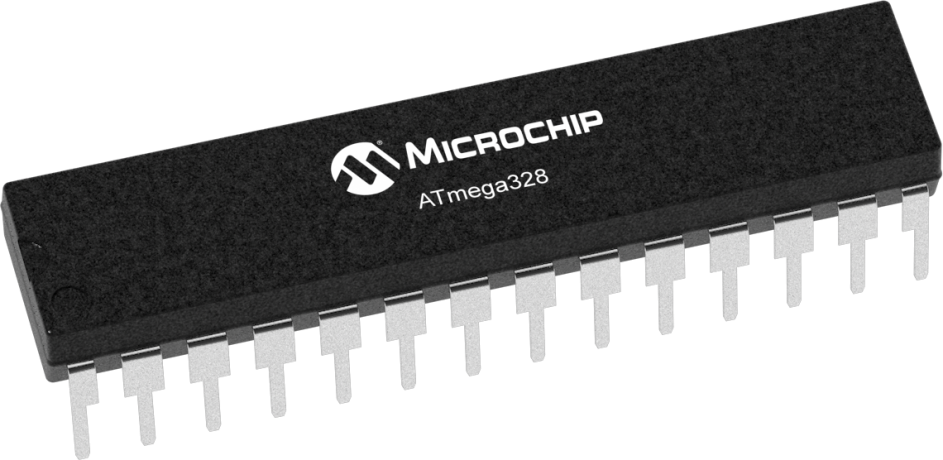
\includegraphics[width=0.25\textwidth]{medium-ATmega328-SPDIP-28.png}
    \captionof{figure}{A Microchip}
    \label{fig:microchip}
\end{wrapfigure}

A microcontroller is a really small microcomputer on a very small chip, see Figure \ref{fig:microchip}.
These are used in a variety of devices; including robots, vending machines, phones, computers, etc. \\

Arduino's are a development board; consisting of an microcontroller, power regulation, and input/output (also known as IO) pins. As microcontrollers are very tiny prototyping with them or using them to build something would be really difficult. The purpose of an arduino is to provide a medium that allows easy development with microcontrollers. There are many different kinds of arduinos, each using a different microchip. \\

\begin{wrapfigure}[10]{r}{0.35\textwidth}
    \centering
    \vspace{-0.5cm}
    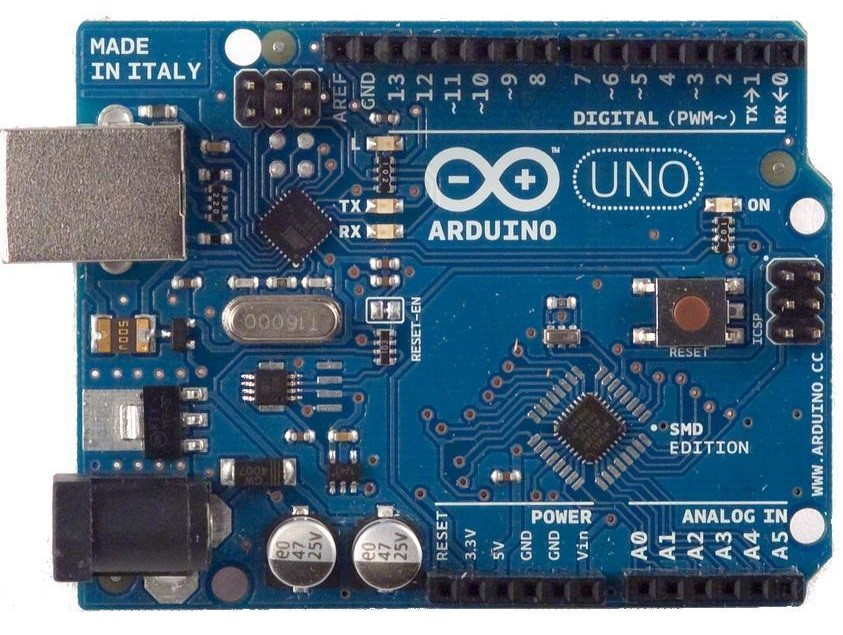
\includegraphics[width=0.3\textwidth]{arduino-uno.jpg}
    \caption{An Arduino Uno}
    \label{fig:arduino-real}
\end{wrapfigure}


The Arduino used in this project is the Arduino Uno, which has an ATMega328p microchip as shown in Figure \ref{fig:microchip}. Figure \ref{fig:arduino-real} is what a real Arduino Uno looks like, though the colour and text may be different from brand to brand. Genuine Arduinos are quite expensive, and there are many clones available which are much cheaper. Figure \ref{fig:arduino-pinout} shows a stylised view of an Uno, labelling all the different pinouts. \\

Arduino's and other development boards are used extensively by hobbyists, they are cheap, easy to use, and extremely versatile. Arduino's are used in nearly every CRoC project, and can be used in countless DIY projects. \\


An Uno has many different ports and pins. Figure \ref{fig:arduino-pinout} shows and labels all the different ports on a standard Uno. \\

An important distinction to make is between the pins 5V, 3.3V, and VIN. VIN stands for voltage in; and this port is used to supply power to the arduino from batteries. Power can also be supplied through the barrel jack connection, see the black rectangle like block on figure \ref{fig:arduino-pinout}. 

The 5V and 3.3V  pins supply 5 volts or 3.3 volts respectively for powering other commponents, such as LEDs, ICs, or sensors.  

\begin{warningbox}
    Never put supply voltage into the 3.3V or 5V pins; this will break the Arduino. 
\end{warningbox}


\begin{center}
    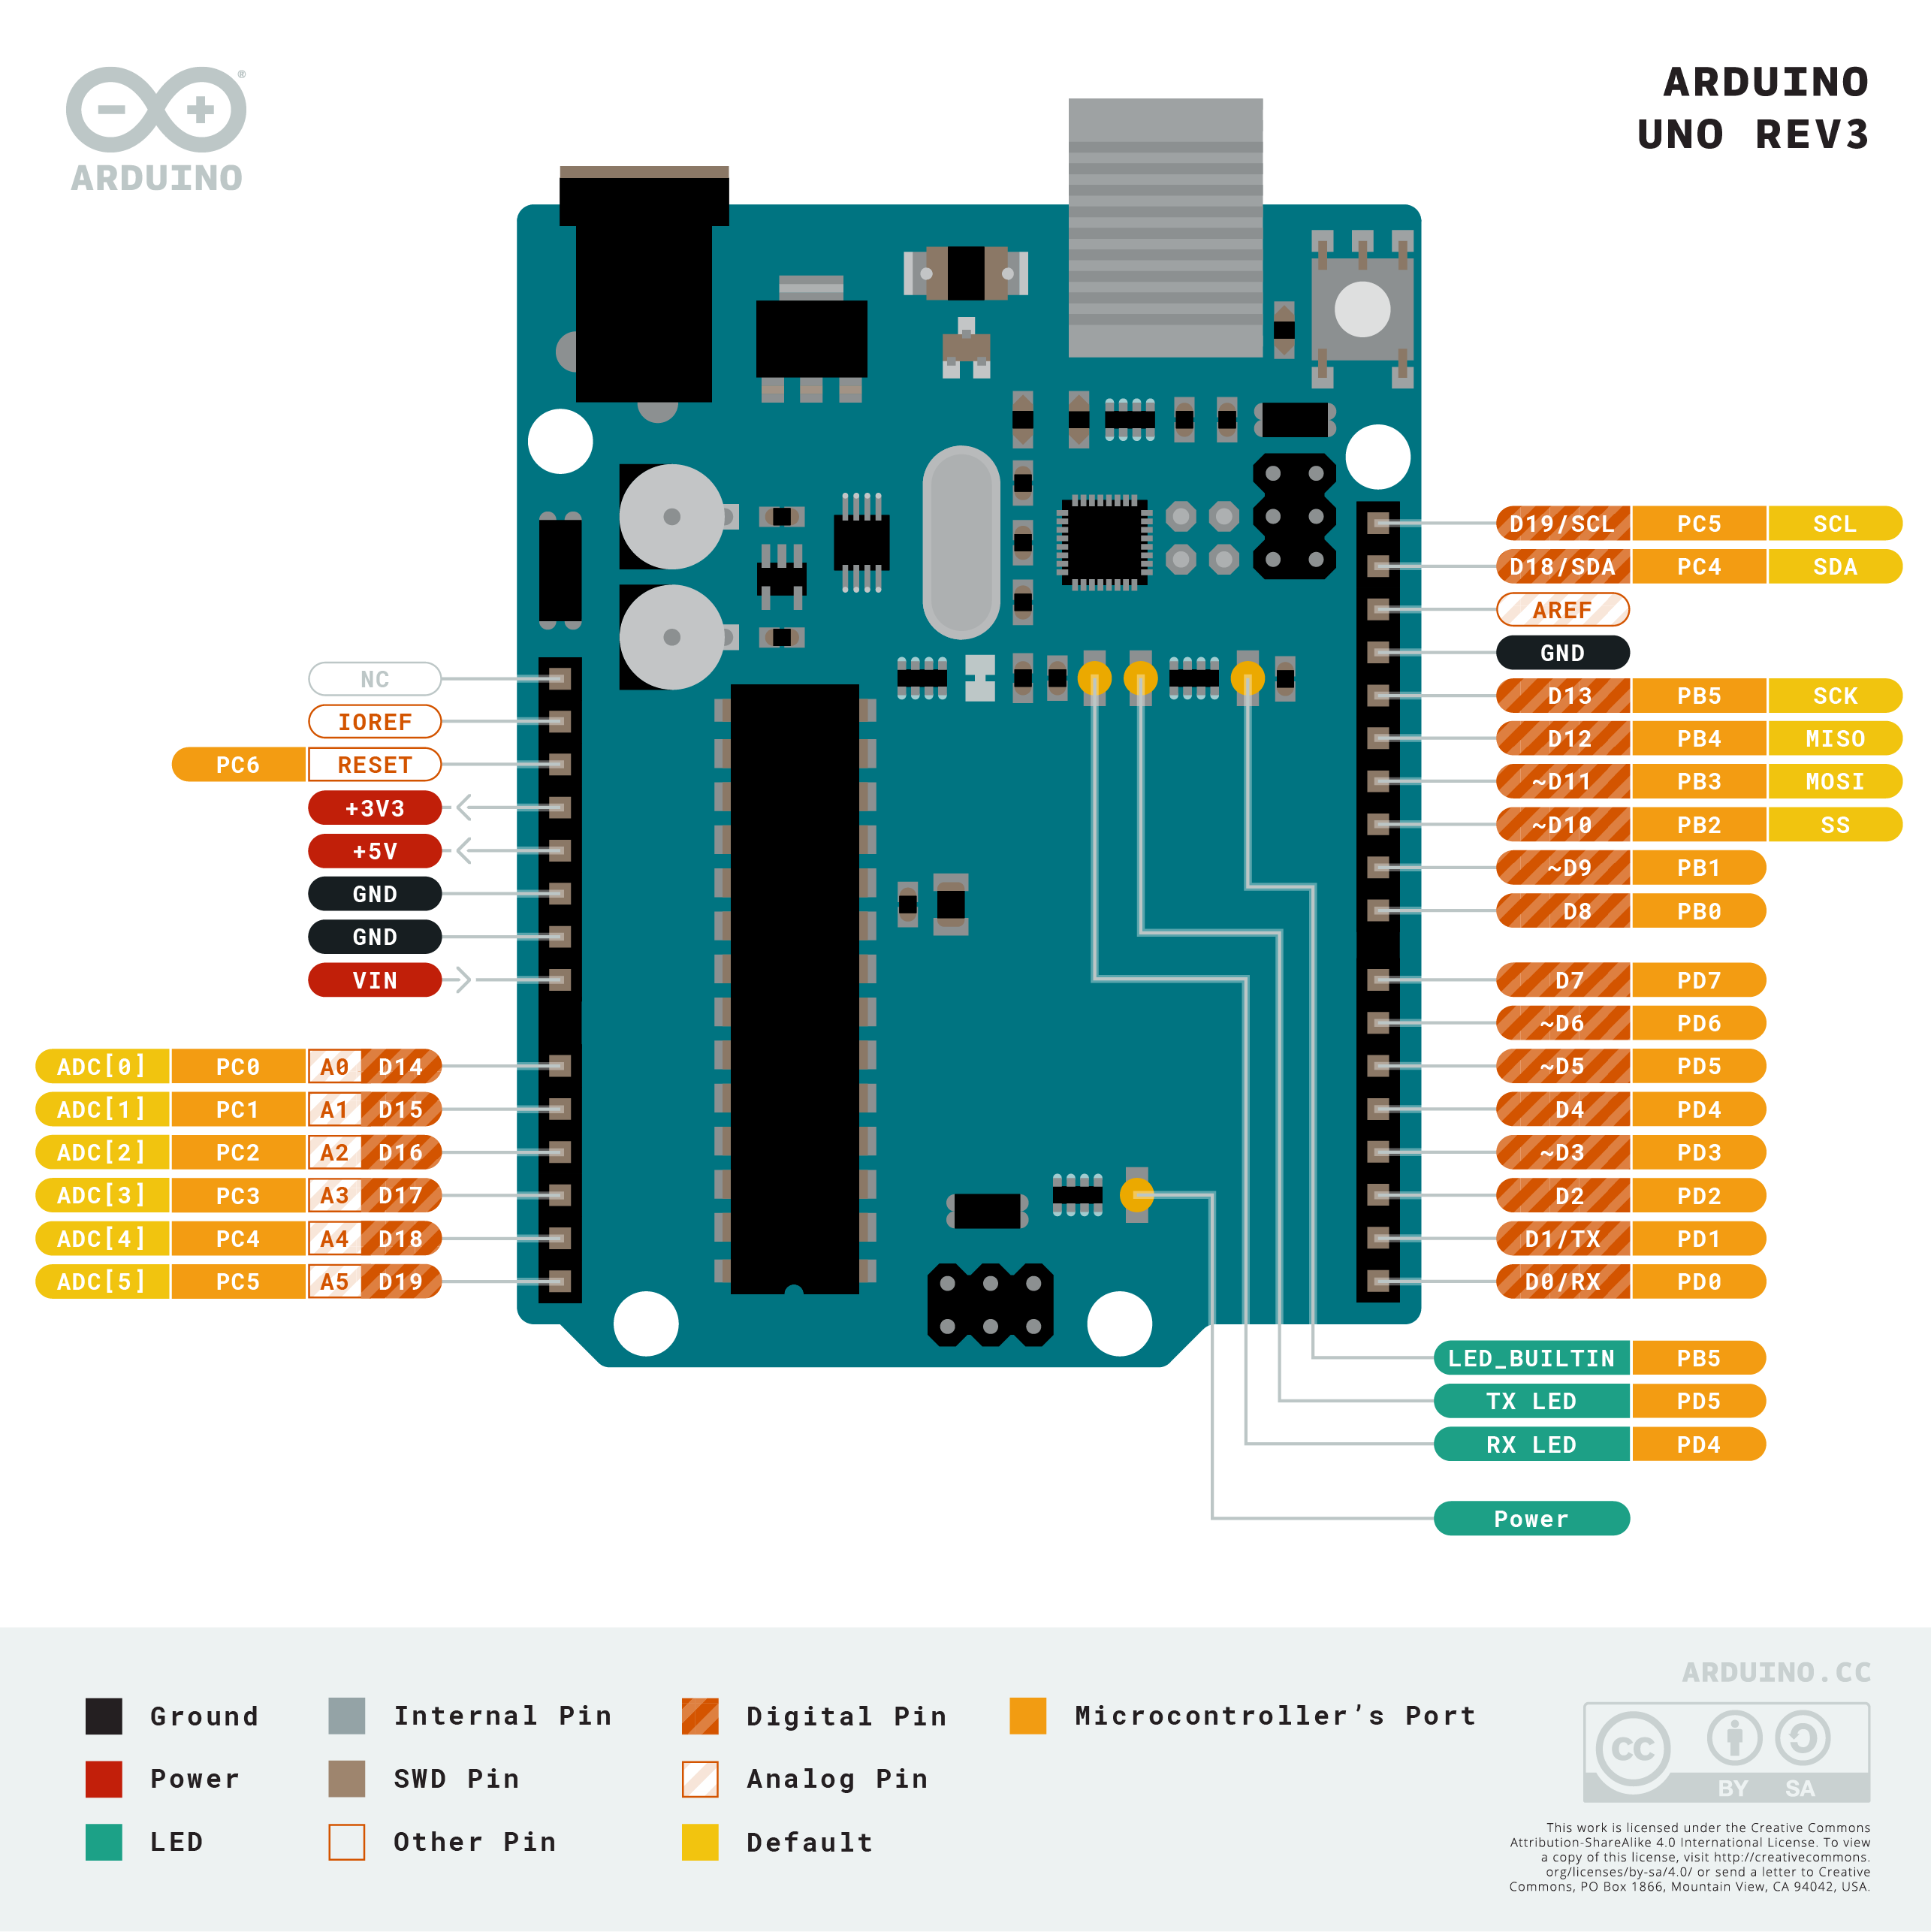
\includegraphics[width=0.8\linewidth]{Pinout-UNOrev3_latest.png}
    \captionof{figure}{Pinout of Arduino Uno}
    \label{fig:arduino-pinout}
\end{center}





\section{Motor} \label{sec:motor}
gearbox, motor

\pagebreak
\section{Motor Controller}

The motors used in this guide, the N20 motors, have a stall current of 1.6A (see section \ref{sec:motor} for what stall current means). The digital pins on an Arduino Uno supply at most 40mA. This is not enough to power the motors.\\ 

To get around this, the Arduino instead interfaces with a \textbf{motor controller}. Motor controllers have a seperate power supply that can supply enough current to drive the motor. Motor controllers also have digital inputs that allow control of the motor. \\


An added benefit of using a motor controller is that it is possible to control the direction, and the speed of the motor. 

\bigskip

The phrase motor controller is often used as a generic term for any device, circuit, or IC which controls a motor. However, motor controllers are a circuit that consists of a motor driver, and some digital harness that acts as an interface to the driver. Motor controllers can be dropped into a circuit and easily controlled, allowing feedback from the motor and more control than a simple driver provides. \\


\subsection{Motor Driver}
A basic motor-\textbf{driver} is a H-bridge. The simplest H-bridge is shown in the below schematics, as well as an explanation of how using a H-bridge allows control over the motors direction. 

\begin{center}
    \begin{circuitikz}
    \draw (0,2) -- (0,0) to
        (0,0) to[nos, l^=$1$] (2,0) to
        (2,0) to [nos, l^=$2$] (4,0) to
        (4,0) -- (4,2) to
        (4,2) to[nos, l^=$3$] (2,2) to
        (2,2) to[nos, l^=$4$] (0,2);
    \draw (2,1) node[elmech](motor){M};
    \draw (motor.north) -- (2,2);
    \draw (motor.south) -- (2,0);
    \draw (0,1) -- (-1,1) node[vee]{};
    \draw (4,1) -- (5,1) node[ground]{};
    % \draw (2,0) to[sV, color=white, name=M] (2,2);
    % \mymotor{M}{90};
    % \draw[rotate=2] (0,2) \mymotor{M}{90} (2,2);
    \end{circuitikz}
    % \captionof{figure}{}
\end{center}

When switches $1$ and $3$ are closed, the current will flow through the motor making it turn anticlockwise.
% in the motor will flow in one direction. 

\begin{center}
    \begin{circuitikz}
        \draw (0,2) -- (0,0) to
            % (0,0) to[o-o, l_=$1$] (2,0) to
            (0,0) -- node[above, yshift=1.5mm]{1} (2,0) to
            (2,0) to [nos, l^=$2$] (4,0) to
            (4,0) -- (4,2) to
            % (4,2) to[l_=$3$] (2,2) to
            (4,2) -- node[below, yshift=-1.5mm]{3} (2,2) to
            (2,2) to[nos, l^=$4$] (0,2);
        \draw (motor.north) -- (2,2);
        \draw (motor.south) -- (2,0);
        \draw[color=red!100, thick] (0,1) -- (-1,1) node[vee]{};
        \draw[color=red!100, thick] (4,1) -- (5,1) node[ground]{};
     
        \begin{scope}[>=latex]
            \draw[->, color=red!100, thick] (-1,1) -- (0,1);
            \draw[->, color=red!100, thick] (0,1) -- (0,0);
            \draw[->, color=red!100, thick] (0,0) -- (2,0);
            \draw[->, color=red!100, thick] (2,0) -- (2,2);
            \draw[->, color=red!100, thick] (2,2) -- (4,2); 
            \draw[->, color=red!100, thick] (4,2) -- (4,1);
        \end{scope}
        \draw (2,1) node[elmech](motor){M};
        \centerarc[->](2,1)(-45:45:0.7);
        \centerarc[->](2,1)(135:225:0.7);
    \end{circuitikz}
\end{center}

In the same vein, closing switches 2 and 4 will cause the motor to turn clockwise. 
\begin{center}
    \begin{circuitikz}
        \draw (0,2) -- (0,0) to
            (0,0) to[nos, l^=$1$] (2,0) to
            % (2,0) to [nos, l_=$2$] (4,0) to
            (2,0) -- node[above, yshift=1.5mm]{2}(4,0) to 
            (4,0) -- (4,2) to
            (4,2) to[nos, l^=$3$] (2,2) to
            % (2,2) to[nos, l_=$4$] (0,2);
            (2,2) -- node[below, yshift=-1.5mm]{4} (0,2);
        \draw (motor.north) -- (2,2);
        \draw (motor.south) -- (2,0);
        \draw[color=red!100, thick] (0,1) -- (-1,1) node[vee]{};
        \draw[color=red!100, thick] (4,1) -- (5,1) node[ground]{};

        \begin{scope}[>=latex]
            \draw[->, color=red!100, thick] (-1,1) -- (0,1);
            \draw[->, color=red!100, thick] (0,1) -- (0,2);
            \draw[->, color=red!100, thick] (0,2) -- (2,2);
            \draw[->, color=red!100, thick] (2,2) -- (2,0);
            \draw[->, color=red!100, thick] (2,0) -- (4,0); 
            \draw[->, color=red!100, thick] (4,0) -- (4,1);
        \end{scope}
        \draw (2,1) node[elmech](motor){M};

        \centerarc[->](2,1)(45:-45:0.7);
        \centerarc[->](2,1)(225:135:0.7);

    \end{circuitikz}
\end{center}

If pins 4 \& 3 or pins 1 \& 2 are closed at the same time, a short circuit will be formed and the H-bridge will break. \\

\begin{minipage}{0.5\textwidth}\vspace{0pt}
    \begin{center}
        \begin{circuitikz}
            \draw (0,2) -- (0,0) to
                (0,0) to[nos, l^=$1$] (2,0) to
                (2,0) to [nos, l^=$2$] (4,0) to
                % (2,0) -- node[below, yshift=-1.5mm]{2}(4,0) to 
                (4,0) -- (4,2) to
                % (4,2) to[nos, l_=$3$] (2,2) to
                % (2,2) to[nos, l_=$4$] (0,2);
                (4,2) -- node[below, yshift=-1.5mm]{3} (2,2) to
                (2,2) -- node[below, yshift=-1.5mm]{4} (0,2);
            \draw (motor.north) -- (2,2);
            \draw (motor.south) -- (2,0);
            \draw[color=red!100, thick] (0,1) -- (-1,1) node[vee]{};
            \draw[color=red!100, thick] (4,1) -- (5,1) node[ground]{};
            
            \begin{scope}[>=latex]
                \draw[->, color=red!100, thick] (-1,1) -- (0,1);
                \draw[->, color=red!100, thick] (0,1) -- (0,2);
                \draw[->, color=red!100, thick] (0,2) -- (2.1,2);
                \draw[->, color=red!100, thick] (2,2) -- (4.01,2);
                % \draw[->, color=red!100, thick] (2,0) -- (4,0); 
                \draw[->, color=red!100, thick] (4,2) -- (4,1);
            \end{scope}
            \draw (2,1) node[elmech](motor){M};
    
        \end{circuitikz}
    \end{center}

\end{minipage}
\begin{minipage}{0.5\textwidth}\vspace{0pt}
    \begin{center}
        \begin{circuitikz}
            \draw (0,2) -- (0,0) to
                % (0,0) to[nos, l_=$1$] (2,0) to
                % (2,0) to [nos, l_=$2$] (4,0) to
                (0,0) -- node[above, yshift=1.5mm]{1}(2,0) to 
                (2,0) -- node[above, yshift=1.5mm]{2}(4,0) to 
                (4,0) -- (4,2) to
                (4,2) to[nos, l^=$3$] (2,2) to
                (2,2) to[nos, l^=$4$] (0,2);
                % (2,2) -- node[above, yshift=1.5mm]{4} (0,2);
            \draw (motor.north) -- (2,2);
            \draw (motor.south) -- (2,0);
            \draw[color=red!100, thick] (0,1) -- (-1,1) node[vee]{};
            \draw[color=red!100, thick] (4,1) -- (5,1) node[ground]{};    
    
            \begin{scope}[>=latex]
                \draw[->, color=red!100, thick] (-1,1) -- (0,1);
                \draw[->, color=red!100, thick] (0,1) -- (0,0);
                \draw[->, color=red!100, thick] (0,0) -- (2.1,0);
                % \draw[->, color=red!100, thick] (2,2) -- (2,0);
                \draw[->, color=red!100, thick] (2,0) -- (4,0); 
                \draw[->, color=red!100, thick] (4,0) -- (4,1);
            \end{scope}
            \draw (2,1) node[elmech](motor){M};
    
        \end{circuitikz}
    \end{center}
\end{minipage}

\bigskip \bigskip

Breaking a H-bridge is fairly common, especially the cheaper low power ones. Some higher end H-bridges are designed to prevent the H-bridge from shorting if the wrong pins are closed. 
Most motor-controllers will have this protection built-in, though most motor-drivers do not. 

\bigskip


% In the case of the H-bridge, the voltage supplied (from the left on the diagrams displayed above) is a high enough voltage, with a high enough current, to drive the motor. The switches (1, 2, 3, 4) are, in their simplest form, a button that is closed upon a signal from the microcontroller. Switches require a very small amount of power to close, and so can be controlled directly from the motor controller. 


\subsection{Motor Controller}



\section{Driving}



\end{document}